\section{Gestion financiera}

\subsection{El negocio de Twitter}

El negocio de Twitter es bastante simple y consta de 3 segmentos:

\begin{itemize}


\item Usuarios: la propuesta de valor de Twitter consisten en ofrecer a su masa crítica de usuarios servicios de microblogging y la posibilidad de mantenerse actualizado de lo que sucede en el mundo  al  instante  a  través  de  diversos  canales  como  su  app  para  smartphones,  su  página web, y las APIs que permiten integrar Twitter en otras webs. Twitter no genera ingresos de manera directa con sus usuarios.

\item Empresas: Aprovechando la masa crítica de usuarios existentes, y la información que posee de  los  mismos,  Twitter  ofrece  servicios  de  publicidad  a  empresas,  que  pueden  mostrar  su publicidad a aquellos usuarios con mayor probabilidad  de  comprar  productos  de  esas empresas (Targeted  Marketing). Estos servicios de Marketing incluyen: tweets promocionados (el anunciante paga por mostrar el tweet a un segmento de usuarios definido), cuentas promocionadas (el anunciante paga por adquirir seguidores) y tendencias promocionadas (el anunciante paga por tener más visibilidad como "trending topic"). Twitter obtiene ingresos de este segmento de clientes.

\item Desarrolladores: Twitter permite además a desarrolladores la posibilidad de conectarse a 
Twitter para generar herramientas relacionadas con analítica web, u otras apps que ayuden a 
hacer crecer la masa crítica de usuarios que utilizan Twitter. Esto aumenta los ingresos de Twitter de manera indirecta. El modelo de negocio de Twitter es un modelo de negocio bilateral, que se basa captar por un lado a usuario que generen actividad y compartan información para su plataforma, y  captar anunciantes por el otro, aprovechando su plataforma y la información generada por sus usuarios para vender servicios de publicidad. Es decir que Twitter actúa como intermediario, como si de una plataforma  de  publicidad  se  tratase.


\end{itemize}

Por tanto, Twitter será rentable en la medida en la que lo sea para sus anunciantes.
Twitter necesita que el valor de cada usuario a lo largo de su vida sea mayor que su coste de adquisición.

\newpage

\subsection{Ingresos y pérdidas (2018)}

\begin{figure}[!htb]
\centering
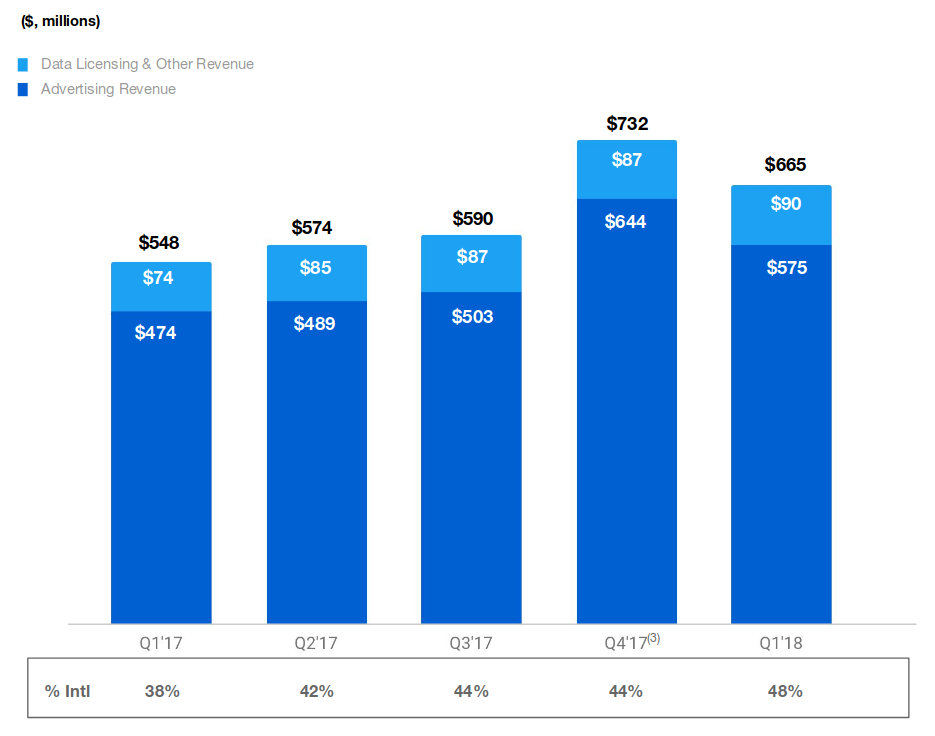
\includegraphics[scale=0.35]{revenues.png}
\caption{\label{fig:frog}Ingresos de Twitter, Inc por cuatrimestres}
\end{figure}

En esta imagen podemos observar cómo los ingresos de Twitter dependiendo de su origen (Licencia de datos, ingresos por publicidad y otros ingresos)


\begin{figure}[!htb]
\centering
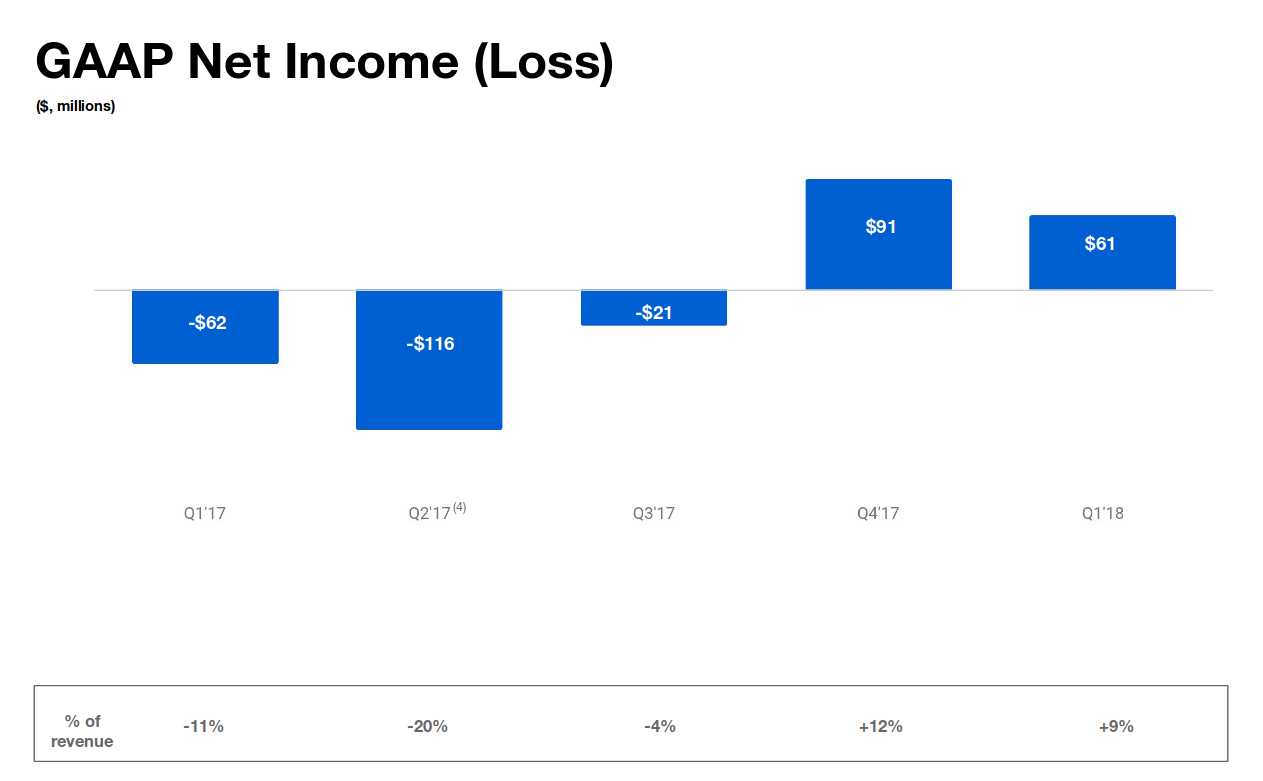
\includegraphics[scale=0.25]{loss.png}
\caption{\label{fig:frog}Ingresos netos de Twitter, Inc por cuatrimestres.}
\end{figure}


Podemos observar cómo los ingresos netos de Twitter Inc. durante comienzos de 2017-2018, fuerosn enteramente negativos.

\subsection{Activos.}

\subsubsection{Activos no corrientes.}

Para Twitter, Inc. los activos no corrientes corresponden a toda su infraestructura de servidores, software, patentes, licencias y datos obtenidos en sus productos.

\subsubsection{Activos corrientes.}

Corresponden al conjunto de bienes de la empresa, en este caso, corresponderá a una parte pequeña de los activos, aunque se espera un crecimiento en esta, ya que como hemos comentado, Twitter, Inc. se encuentra en una etapa de madurez a nivel empresarial, lo que resultara en una generación de beneficios.


\subsection{Recursos financieros.}

\begin{figure}[!htb]
\centering
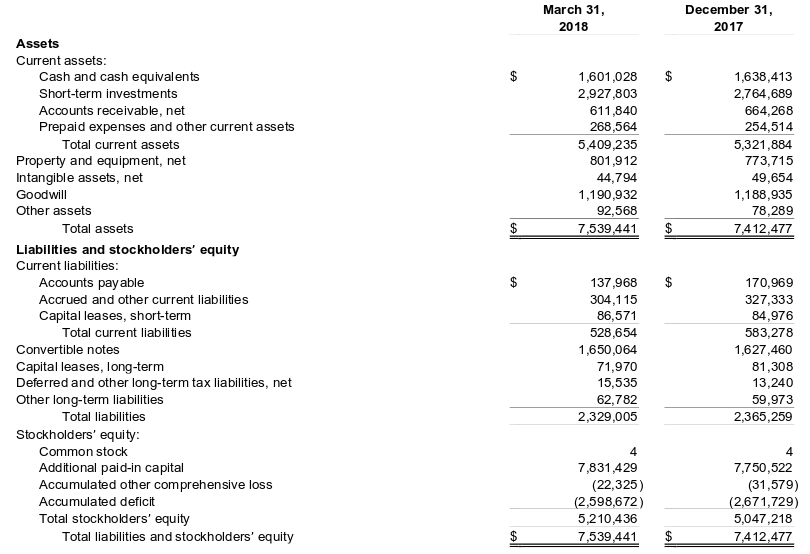
\includegraphics[scale=0.6]{ingresos.png}
\caption{\label{fig:frog}Diferencia de ingresos de Twitter, Inc.}
\end{figure}

\subsubsection{Recursos financieros propios.}

Como vemos en la imagen de ingresos de Twitter, Inc. , menos de la mitad de ingresos que usa Twitter, Inc. son generados  por la empresa, esto es causado por el ámbito de esta, ya que normalmente, en las empresas de ámbito tecnológico el valor de la empresa viene dado por la importancia que el sector le de a esta, ya que los propios productos no pueden ser evaluados de forma física.

\subsubsection{Recursos financieros externos.}

La inversión de agentes externos en la empresa tiene una gran importancia, de ahí que se generen grandes conflictos de intereses en Twitter, Inc. , los valores de la compañía difieren con los valores de los stakeholders, aunque la estructura organizativa permita lidiar con estos.

\subsubsection{Fondo de maniobra.}

Observamos como el fondo de maniobra ha sido muy importante para Twitter, Inc. ya que ha permitido mantener la empresa en su etapa anterior, en la que no era capaz de generar ingresos netos. Se espera que en un periodo de tiempo próximo (a corto plazo) este fondo se amplié gracias al comienzo de generación de ingresos.

\section{Recursos Humanos}

A grandes rasgos, los recursos humanos de una empresa son el conjunto de empleados y colaboradores que
trabajan en la empresa, aunque comunmente nos referimos a ellos como el proceso de reclutamiento, selección, formación, evaluación, compensación... de una empresa. Normalmente, estas políticas son llevadas a cabo por un departamento en específico dentro de la empresa.

\subsection{Reclutamiento}

En Twitter, el reclutamiento es un proceso muy sencillo, ya que en su misma página principal te dan la opción de presentarte para poder trabajar con ellos en sus diferentes departamentos en sucursales de todo el mundo.


\includegraphics[scale=0.25]{reclutamiento1.png}

Una vez accedida a esta sección, decides a qué departamento quieres aplicar para pasar al proceso de selección.


\includegraphics[scale=0.25]{reclutamiento2.png}

\subsection{Selección}

El proceso de selección en Twitter, Inc. consta de 3 pasos

\subsubsection{Paso 1}
Después de presentar la solicitud, un reclutador podría comunicarse con el solicitante para efectuar una llamada de presentación.

\subsubsection{Paso 2}
Si es del agrado del reclutador, más tarde le llamarán para entrevistas con una o dos personas más.

\subsubsection{Paso 3}
Si continua a lo largo del proceso, irá a la oficina de Twitter (En el lugar solicitado por el solicitante) una o dos veces para entrevistarse finalmente con 5-10 personas más.

\subsection{Compensación}

Twitter se preocupa del estado en el que sus empleados trabajan, por tanto, para retener el talento, se centran en dos puntos: el aprendizaje y la directiva.
En la empresa tienen organizaciones de aprendizaje de talla mundial enfocadas a Twitter. Tienen Twitter University, enfocado al desarrollo de capacidades de ingeniería móvil para los empleados de la compañía. Por otro lado, creen que la clave para la comodidad de sus empleados es que sus directores sean personas competentes y agradables, por ello, los directores de departamento reciben 6 horas de clase de dirección y motivación al trimestre, de esta manera, los directores estarán implicados y apasionados realmente en el proyecto. En Twitter Inc piensan que no se despiden puestos, sino empleados.

\subsection{Formación}

Como hemos comentado anteriormente, existe una formación interna tanto como para empleados, como para directivos llamada Twitter University.

\subsection{Socialización}

Para facilitar el proceso de adaptación de un nuevo trabajador a la empresa, Twitter ofrece en sus oficinas lugares de ocio como salones y comedores donde los empleados pueden relacionarse y descansar tras una jornada de trabajo.

\subsection{Relaciones Laborales}

La directora de Recursos Humanos afirma que la clave del éxito en este ámbito es, sin duda, el apoyo que brindan los directores a los empleados de sus proyectos, por tanto, hay una estrecha relación entre todos los trabajadores de la empresa.

\section{El Marketing}

Definimos Marketing como: $"$Conjunto de técnicas y estudios que tienen como objeto mejorar la comercialización de un producto$"$.

A continuación explicaremos cómo aborda Twitter las actividades de Marketing.

\subsection{Análisis de Mercado y comportamiento del consumidor}

Twitter se encuentra en un sector muy competitivo: las redes sociales.

Existen muchas aplicaciones de comunicación de este tipo, como Facebook, Instagram, Snapchat, Tumblr... ¿Pero qué es lo que ha hecho a Twitter destacar ante sus competidores?

Twitter se dirige a un mercado joven y dinámico, pero también con el paso del tiempo, se ha transformado en una herramienta para las empresas, tanto para promocionarse y anunciarse como para investigar el comportamiento y preferencias de su clientela.
La clave de su éxito reside en la facilidad de uso que tiene (tanto para publicar tu propio contenido como para interactuar con el contenido ajeno), la posibilidad de personalización, el uso de los llamados \textit{hashtags} para agrupar contenidos, la ausencia de censura exceptuando 5 países y, para atraer visitas y ver de qué se habla en el momento, las \textit{tendencias}.

Nuestra empresa ha sabido localizar el centro de su público y darles las herramientas necesarias para expresarse libremente y de forma segura.

\subsection{Estrategia de Marketing}

La nueva estrategia de Marketing de Twitter incluye vídeos explicando los valores que lo distinguen de las otras plataformas. Este resultado se deriva de la investigación que la compañía reveló. Mientras que el 90\% de las personas reconocían globalmente la marca Twitter, no lo usaban porque no entendían qué era Twitter. La compañía busca ahora cambiar la percepción de que Twitter es una red social que permite a los usuarios conectarse con familiares y amigos para convertirse en un lugar activo para descubrir noticias.

Twitter se está posicionando como plataforma única donde se pueden acceder tanto a noticias de grandes eventos, hasta noticias locales junto con comentarios en directo.

Esta estrategia que destaca su singularidad atraerá a más público, afirma la directora de Marketing.

También están haciendo convenios con compañías como Samsung para que su aplicación venga instalada de forma predeterminada en sus dispositivos.